\section{Review of the state-of-the-art}
\label{sec:related-work}
\subsection{QC LDPC bit-level codes}
In general, LDPC encoding refers to the process of calculating the mapping $s \rightarrow c$ of a k-bit binary vector $s\in\{\mathbb{F}_2\}^k$ to the proper element $c$ of the k-dimensional subspace $V\subset\{\mathbb{F}_2\}^n$, according to the code definition, which is defined by the parity-check matrix $H$ of the code, so that the parity-check equation $ cH^{T}=0 $ is satisfied.\par
The encoding methods for LDPC codes can be classified into the following categories:\par
\textbf{\textit{Direct method}}\par
The direct method involves the application of Gaussian elimination to calculate the generator matrix $G$ from the null space of the parity-check matrix $H$ of the code, that is to solve the equation $GH^{T}=0 $. This process takes place offline and depending on the encoder's implementation details, the generator matrix data or structure is stored into the encoder. A codeword $c$ can thus be calculated from the input information block $s$ through the vector-matrix multiplication $c=sG$.\par
In order to facilite encoder design, for all the practical LDPC codes used in modern communications systems, the generator matrix can be calculated in systematic form. For a $(n,k)$ linear block code in this case $G=\begin{bmatrix}I_{k} & W_{n-k}\end{bmatrix} $, where $I_{k}$ is the $k\times k$ identity matrix and for QC codes, $W_{n-k}$ is an array of dense cyclic sub-matrices, with the structure of (\ref{eq:Wstructure}). The resulting codeword $c$ is consequently $c=\begin{bmatrix}s & p\end{bmatrix}$, where $p$ is the vector of the $n-k$ parity bits. In this case, the encoders implementing this method need only to store the $r \times c \times m$ bits of the first rows (or columns) of these circulants. However, despite the fact that the initial parity-check matrix $H$ is sparse, the resulting $W_{n,k}$ matrix and consequently its constituent circulants are dense matrices. In \cite{Mahdi2014}, \cite{Wang2008} and \cite{Lee2004} compression methods are proposed, which reduce the memory requirements to store the circulants of the parity-check matrix $H$ in the encoder. These methods however are not applicable to dense matrices, nor are the corresponding architectures which handle the sparse matrix operations involved in the calculations.\par  
\begin{equation}
    W_{n-k}=
    \begin{bmatrix}
        W_{1,1} & \dots  & W_{1,c} \\
        \vdots  & \ddots & \vdots \\
        W_{r,1} & \dots  & W_{r,c}
    \end{bmatrix}
    \label{eq:Wstructure}                   
\end{equation}
Encoders proposed in \cite{Theodoropoulos2016},\cite{ZhaohuiWangXinHaoChangxingLin2018},\cite{Miles2006},\cite{ZongwangLi2006},\cite{Andrews2005},\cite{Yasotharan2009},\cite{Yen2012}  are based on the direct encoding method. My preliminary  work in \cite{Theodoropoulos2016} has introduced an efficient architecture for the parallel execution of the vector-matrix multiplication involved in the direct encoding method, by leveraging the inherent parallelism of the generator matrix of CCSDS codes, achieving.\par
Although the work in \cite{ZhaohuiWangXinHaoChangxingLin2018} focuses in CCSDS codes, the proposed architecture handles encoding inefficiently, requiring large XOR operations over a significant number of bits ($k/2$ or 2048 in the provided example) and at the same time register resources are wasted. Algorithmically, the approach is also equivalent to \cite{Yasotharan2009} and the parallel SRAA of \cite{ZongwangLi2006}. The required logic resources for hardware implementation are inevitably a large portion of a Virtex7-xc7vx485t FPGA.\par
In \cite{Miles2006}, the problematic dimension of the C2 code at the boundaries of the 511-bit circulants when processing a stream of input data is handled by packing input bits present on the 16-bit input bus into groups of 21-bits and unpacking them subsequently to groups of 7 bits for the AND-XOR operations. The difference however between the size of the input bus (16 bits) and the degree of parallelism in the AND-XOR process (MAC module), leads to suboptimal use of the resources of the MAC module, which remains idle for a number of cycles, when input has starved. Moreover, additional computation cycles are wasted by the 18 trailing zeros which are prepended to the information block, according to C2 code description, which are processed by the MAC module in this particular approach. Our architectures handle these problems in a more efficient way, as described in a subsequent section.\par
The authors in \cite{ZongwangLi2006} propose various types of encoding circuits, based on shift registers, which achieve encoding complexity linearly proportional to the number of parity bits of the code ($n-k $ according to the notation in this work), or the $n$ total bits of the code in the case of the parallel approach. The SRAA serial encoding scheme described is practically the naive approach provided in the CCSDS standard \cite{CCSDS131.0}, based on a shift register for the circulants and a register for the calculation of parity bits. The calculated complexity does not include the memory and the necessary circuitry for the loading of the generators $g_{i,j}$ of the circulants to the SRAA shift registers, which incur significant resources cost in practical implementations, as it will be shown in a subsequent section. According to the parallel SRAA approach, which achieves encoding in $cb$ cycles (following the writers' notation), all $k$ input bits participate in the calculation of each parity bit in one clock cycle. This architecture could not be implemented with reasonable resources in practical encoders for codes with block lengths in the range of several thousands of bits and should be considered only as a theoretical approach for academic research purposes only. Even in this case however, the AND-XOR binary calculations on a large number of bits would necessitate large combinatorial paths and would severely jeopardize throughput performance. The two-stage encoding scheme described is practically the \textit{H2-inverse} method described later in the current Section.\par
The work in \cite{Andrews2005} proposes an architecture based on Linear Feedback Shift Registers (LFSRs). The input information bits are multiplied with the first rows of the circulants $W_{i,j}$ and instead of rotating the circulant registers, the rotation concerns the output register, which contains the parity bits at the end of the encoding process.\par
The approach described in \cite{Yasotharan2009} is algorithmically equivalent to the parallel SRAA approach of \cite{ZongwangLi2006}, without taking advantage of the QC structure of the targeted codes (IEEE 802.16e). Its performance however is also dominated by the large XOR binary operation involved. In addition, the memory requirements for the storage of the generator matrix, totalling $(n-k)k$ bits, pose considerable constrains to the associated hardware. Finally, \cite{Yen2012} is another adoption of the SRAA architecture of \cite{ZongwangLi2006} employing the direct method, optimized for sparse circulants.\par

\textbf{\textit{R-U method}}\par
This method is based on the fact that the codeword can be calculated directly from the H matrix by solving the system of equations defined by the parity-check equation $Hc^{T}=0$. The Richardson-Urbanke (R-U) method \cite{Richardson2001} solves this equation with complexity almost linear to the block length, provided that the parity-check matrix of the corresponding QC-LDPC code has approximate upper-triangular structure, or it can be  transformed to such form, which is depicted in Fig.\ref{fig:RUmatrix}. For a systematic code with a $H$ matrix of size $(n-k)\times k$, the calculated codeword has the form $c=\begin{bmatrix}s & p_{1} & p_{2} \end{bmatrix}$, where $s$ is the input vector and $p_{1}$, $p_{2}$ are parity bits vectors of length $g$ and $m-g$ respectively and and the parity bits are calculated according to (\ref{eq:RUphi}), (\ref{eq:RU1}), (\ref{eq:RU2}).\par
\begin{figure}
    \centering                            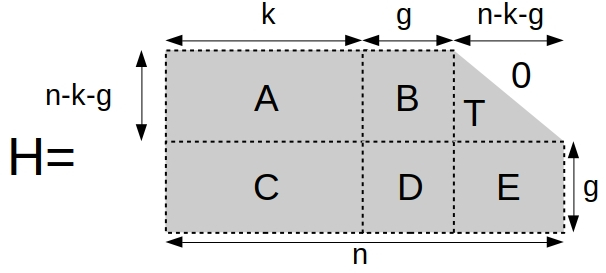
\includegraphics[width=0.4\linewidth]{Figures/RUmatrix.jpg}
    \caption{Structure or H matrix for the R-U method}
    \label{fig:RUmatrix}
\end{figure}
\begin{equation}
    \varphi=ET^{-1}B+D
    \label{eq:RUphi}
    \end{equation}
\begin{equation}
    p_1^{T}=\varphi^{-1}(ET^{-1}A+C)s^{T}
    \label{eq:RU1}
    \end{equation}
\begin{equation}
    p_{2}^{T}=T^{-1}(As^{T}+Bp_1^{T})
    \label{eq:RU2}
\end{equation}

The above equations involve many sparse matrices, but only a single dense, namely $\varphi^{-1}$. Sparse matrix operations can be implemented by simplified hardware and the determinant factor affecting the performance of the encoder becomes the $g \times g$ dense matrix $\varphi^{-1}$. The parity-check matrix of many widely adopted LDPC codes has been specifically designed so that the parameter $g$ is small, or in the case of DVB-S2 is zero and the matrix $\varphi^{-1}$ has a special strucutre which results in efficient hardware implementation. For example, the $\varphi$ matrix of the LDPC codes adopted for IEEE 802.11ac/n, 802.16e and many other applications is the $g \times g$ identity matrix.\par
For many other codes, transformation into approximate lower triangular form, without affecting the QC structure of the matrix is not straightforward. For example, in the case of the CCSDS codes defined in \cite{CCSDS131.0}, this can be achieved by shifting the last 4 circulants ($4m$ bits) by 8 columns ($8m$ bits) to the left. Since the last $4m$ bits of the code are punctured, this permutation does not affect the encoder's output. Fig.\ref{fig:RUH} displays the $H$ matrix before and after the transformation for rate $1/2$ AR4JA code with $k=1024$. The parameter $g$ is therefore $4m$ and $\varphi^{-1}$ is a $4m \times 4m$ dense QC matrix of $m \times m$ circulants.             
Architectures proposed in \cite{Lee2004}, \cite{Tzimpragos2013}, \cite{HaoZhong2005}, \cite{Yu2014}, \cite{Wang2017}, \cite{HaibinZhang2008} are examples of application of the R-U method.\par
          The work in \cite{Lee2004} does not target QC codes, nor can it efficiently handle large dense $\varphi$ matrices. The parameter $g$ is 2 in the provided implementation examples and the resulting encoders occupy a large amount of the resources of Xilinx XC2V4000-6 FPGA, including a number of Block RAMS. The encoder architecture in \cite{Tzimpragos2013} targets IEEE 802.11n codes where $\varphi$ matrix is the identity matrix, but is not applicable to CCSDS codes. Targeting Wimax LDPC codes, \cite{Wang2017} also assumes that $\varphi$ is the identity matrix. In \cite{HaoZhong2005} the authors propose a code construction method, together with encoder-decoder architectures. The proposed encoder implements the R-U method, but the code construction aims at minimizing the parameter $g$. The dense matrix multiplication (\ref{eq:RU1}) involving $\varphi$ in their case is executed on all elements of $\varphi^{-1}$ in parallel, which obviously does not scale efficiently for large $g$. The method proposed in \cite{HaibinZhang2008} and \cite{Yu2014} employs SRAA modules introduced in \cite{ZongwangLi2006} for the dense matrix operations of the RU algorithm. The scalability issues concerning the adoption of SRAA architectures for the direct encoding method, also petrain to the R-U method for CCSDS codes, because of the size of parameter $g$.\par
          %             Fig \ref{fig:phiInv} gives an example for the matrix of the same code. \par 
                \begin{figure}
                \centering
                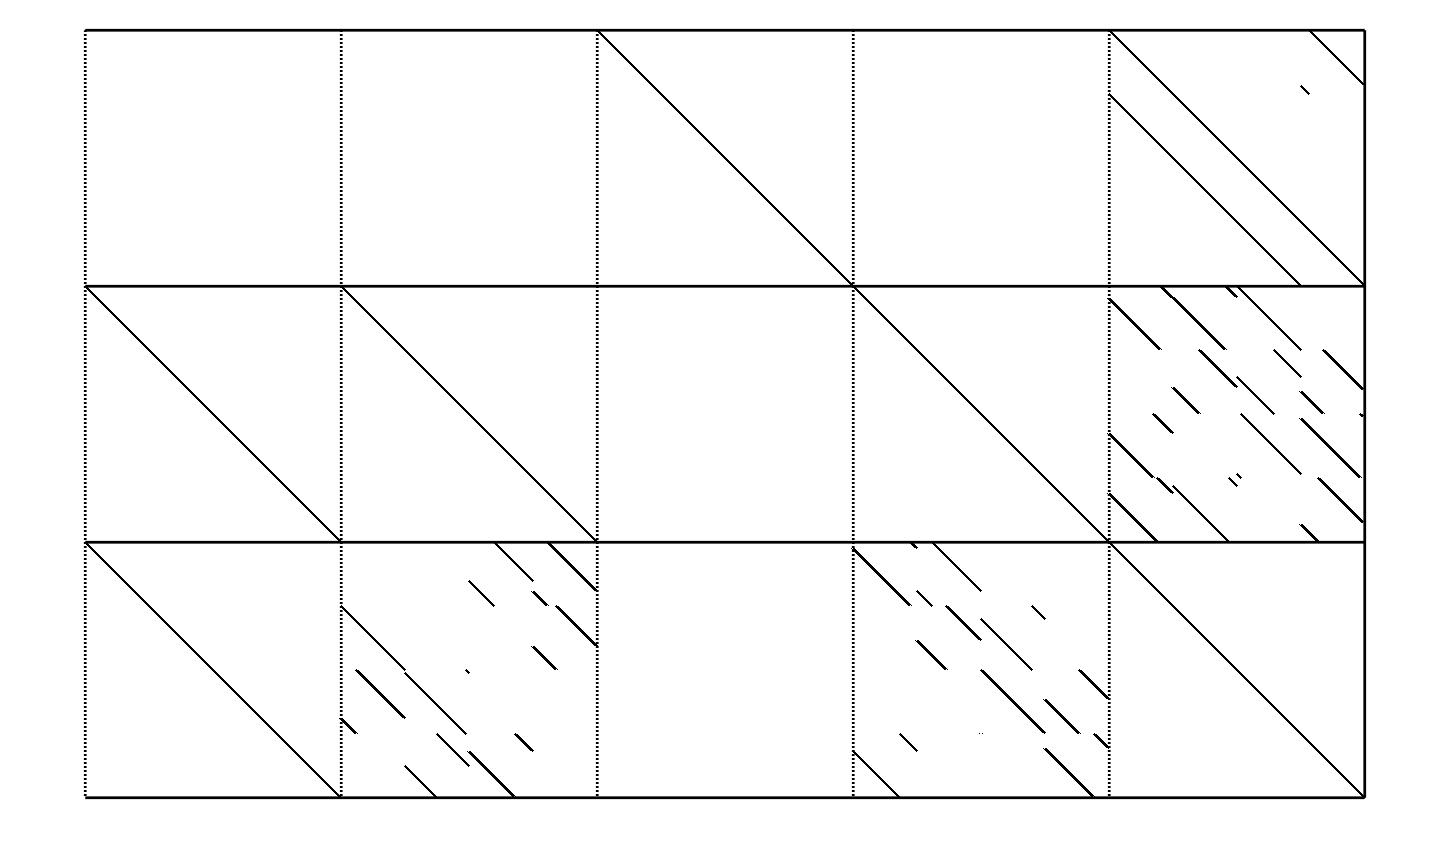
\includegraphics[width=0.4\linewidth]{Figures/HRUa.jpg}
                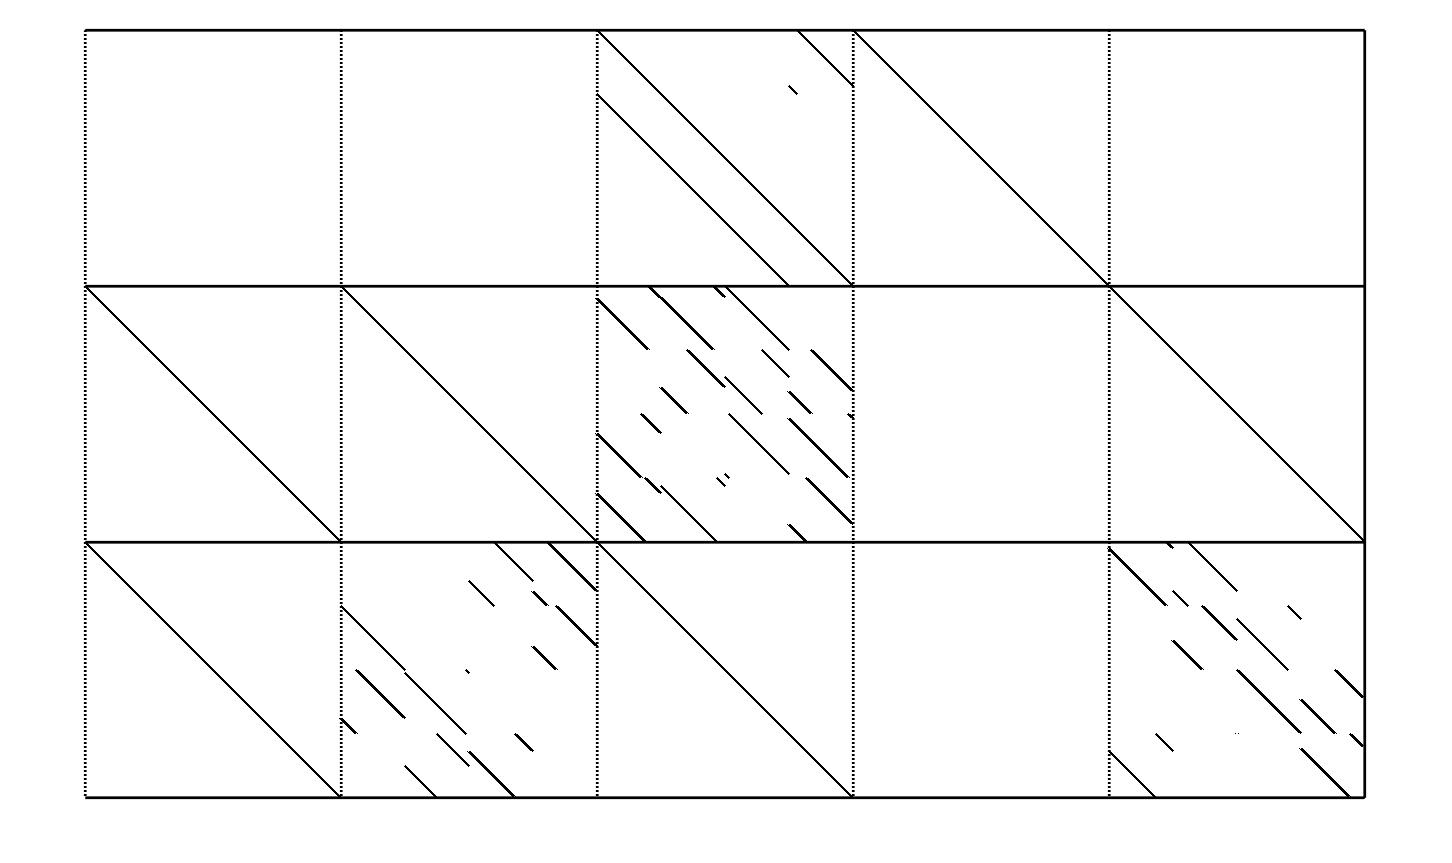
\includegraphics[width=0.4\linewidth]{Figures/HRUb.jpg}
                        \caption{$H$ matrix before (left) and after (right) the transformation into lower triangular form.}
                \label{fig:RUH}
                \end{figure}                    
        %       \begin{figure}
        %       \centering
        %       \includegraphics[width=0.3\linewidth]{Figures/phInv.png}
        %               \caption{$\varphi^{-1}$ submatrix for AR4JA codes $m=128$ bits for this code.}
        %       \label{fig:phiInv}
        %       \end{figure}    
            




\textbf{\textit{Partitioned $H$ methods}}\par
This class of methods is based on the fact that for all systematic codes, the codeword $c$ consists of the systematic part, which is a copy of the input information block and the parity bits: $c=\begin{bmatrix}s & p\end{bmatrix}$. The parity-check matrix can therefore be partitioned into a $(n-k)\times k$ submatrix $H_{1}$ and a $(n-k) \times (n-k)$ submatrix $H_{2}$, where $H=\begin{bmatrix}H_{1} & H_{2}\end{bmatrix}$, so that the parity bits vector can be calculated by (\ref{eq:H2inv1}), (\ref{eq:H2inv2}), (\ref{eq:H2inv2}).
    \begin{equation}
        Hc^{T}=H_{1}s^{T}+H_{2}p^{T}=0
        \label{eq:H2inv1}
    \end{equation}
    \begin{equation}
        H_{2}p^{T}=H_{1}s^{T}
        \label{eq:H2inv2}
    \end{equation}
    \begin{equation}
        p^{T}=H_{2}^{-1}H_{1}s^{T}
        \label{eq:H2inv3}
    \end{equation}
Submatrix $H_1$ is sparse and the vector $H_{1}s^{T}$ can be easily calculated. For many practical codes, submatrix $H_{2}^{-1}$ exhibits regular structure, which facilitates the involved calculations. A common structure in the parity-check matrix of many codes is the dual-diagonal: the rightmost part or of $H_{2}$, or even the entire submatrix (IEEE 802.11 n/ac, 3GPP2 DVB-S2) is a dual-diagonal matrix. \par
According to a variation of this method (\cite{Jia-ningSu2005}, \cite{Kaji2006}), $H_2$ matrix is decomposed into a permutation matrix $\Pi$ and two triangular matrices $L$, $U$, using triangular factorization (or LU decomposition).  Equation (\ref{eq:H2inv2}) is therefore transformed into (\ref{eq:LUH2-2}), from which parity bits are calculated using back-forward substitution. Conversely, the LU decomposition can be applied on $H_{2}^{-1}$ matrix, so that parity bits are calculated according to (\ref{eq:LUH2inv-1}),(\ref{eq:LUH2inv-2}).
                \begin{equation}        
                        H_{2}=\Pi^{-1}(LU)              
                        \label{eq:LUH2-1}
                 \end{equation}                                          
                 \begin{equation}
                         L[U(p^{T})]=\Pi(H_{1}s^{T})
                        \label{eq:LUH2-2}
                 \end{equation}  
                 \begin{equation}       
                        H_{2}^{-1}=\Pi'^{-1}(L'U')              
                        \label{eq:LUH2inv-1}
                 \end{equation}  
                 \begin{equation}
                        \Pi' p^{T}=L'[U'(H_{1}s^{T})]
                        \label{eq:LUH2inv-2}
                 \end{equation}
 The architectures proposed in \cite{Gomes2007}, \cite{AlHariri2013}, \cite{ZhiyongHe2006}, \cite{Hariri2014}, \cite{Perez2010a} and \cite{YongminJung2012} all follow algorithmically equivalent approaches which assume a dual-diagonal $H_2$ matrix. Parity bits can be calculated directly from the vector $H_{1}s^{T}$ using backward substitution. In  (\ref{eq:H2inv3}), $H_{2}^{-1}$ is a lower triangular matrix and $H_{2}^{-1}(i,j)=1, i\geq j$, so that back substitution is applicable.\par
For another class of codes (for example in IEEE 802.16e), $H_2^{-1}$ has the approximate dual-diagonal structure of (\ref{eq:ApproxDual}), where $I_{i}^{(x_{j})}$ are permutation matrices. Targeting these cases, \cite{Neto2015}, \cite{Kopparthi2007} and \cite{Chia-YuLin2008} propose  encoders with similar algorithmical description, which perform necessary permutations along with backward substitution for the calculation of the coresponding parity bits.\par         
    \begin{equation}
        H_{2}^{-1}=\left[
        \begin{array}{c|ccccc}
        I_{1}^{(x_{1})} & I & I & \dots &       0    & 0\\
        \vdots & & & \dots \\
        I_{b}^{(x_{b})} & 0 & 0 & \dots & I & I\\
        \end{array}\right]
    \label{eq:ApproxDual}
    \end{equation}\par
For many codes however (including those in \cite{CCSDS131.0}), $H_{2}^{-1}$ matrix has the structure of (\ref{eq:H2InvStruct}), where $0_{4m}$ and $I_{4m}$ are the $4m \times 4m$ zero and identity matrices and $W_{i,j}$ are $m \times m$ dense circulants, which is obviously not dual-diagonal, rendering the above architectures altogether inapplicable.
    \begin{equation}
        H_{2}^{-1}=
        \begin{bmatrix}
            I_{4m} & W_{1,1} & \dots  & W_{1,8} \\
            0_{4m} & \vdots  & \ddots & \vdots \\
            0_{4m} & W_{12,1} & \dots  & W_{12,8}
        \end{bmatrix}
        \label{eq:H2InvStruct}                  
    \end{equation}\par
The variation of the method based on L-U decomposition of $H_{2}$ according to (\ref{eq:LUH2-1})-(\ref{eq:LUH2inv-2}) is used in \cite{Jia-ningSu2005}, where the authors also propose an offline preprocessor for the triangulation of $H_{2}$. The QC structure of the matrix however is not kept in the decomposed matrices, at least for the demonstrated codes. Reference \cite{XiangranSun2011} proposes the same encoder architecture with a different decomposition algorithm for CMMB codes, which are not QC. The same encoder architecture is also proposed for CMMB in \cite{Wang2008}, without details on the decomposition algorithm. The work in \cite{Kaji2006} targets random Gallager codes. The encoding process is identical to \cite{Jia-ningSu2005}, however algorithms are provided for the calculation of permutation matrices, which minimize the density of $L$, $U$ components. It is shown that the compression achieved for the storage of sparse $L$, $U$ matrices favors this method over R-U, at least for Gallager codes. The adoption of this encoding method however for CCSDS inflicts a major performance penalty because of the loss of QC structure in $L$, $U$ matrices. For example, using the triangulation process outlined in \cite{Jia-ningSu2005}, the AR4JA rate $1/2$ code with $k$=1024 bits calls for the storage, proper indexing and processing of a total of around 64K nonzero elements of $L$, $U$ matrices, compared to the simple storage of the 2K elements of the first rows of the circulants needed for the $4m \times 4m$ $\varphi^{-1}$ matrix.\par               
The work in \cite{Mahdi2014} modifies the procedure in \cite{Jia-ningSu2005} and adopts LU decomposition of $H_{2}^{-1}$, so that parity bits are calculated according to (\ref{eq:LUH2inv-2}). It is shown that for the selected codes (Multi-level QC-LDPC codes), this method can result in more efficient storage of $L'$, $U'$ and $\Pi'$ in the encoder's memory than $H_{2}^{-1}$ or storing the components of $H_{2}$ according to \cite{Chia-YuLin2008}. However, the efficiency of the proposed encoding scheme is limited only to the two-step expanded codes, which results in cyclic structure in the triangulated components. Fig.\ref{fig:Mahdi-LU} depicts an example of the generated $L'$ and $U'$ matrices, compared to their CCSDS equivalents. The VMM architectures proposed for the vector-matrix multiplications are evidently not applicable for the random matrices of CCSDS. Memory requirements for indexing the non-zero values are also a considerable drawback. Another fully parallel method is also proposed, targeting high throughput. According to this method, there is no need to store $L'$, $U'$ in memory and the vector-matrix multiplications of (\ref{eq:LUH2inv-2}) are executed in parallel on all bits. This method cannot scale for higher block lengths or other codes. Even for CCSDS AR4JA $k$=1024, rate $1/2$ code, the implementation of this method required more than 72K LUTs, fitting only high-end Virtex 5 FPGAs, with prohibitive routing delays for any practical application.\par
\begin{figure}
    \centering
    
\includegraphics[width=0.24\linewidth]{Figures/LMahdi.png}
    
\includegraphics[width=0.24\linewidth]{Figures/UMahdi.png}
    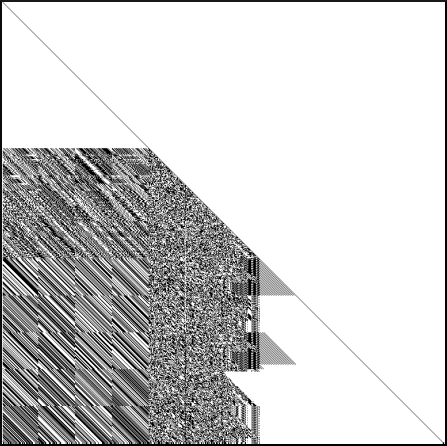
\includegraphics[width=0.24\linewidth]{Figures/LAR4JA.png}
    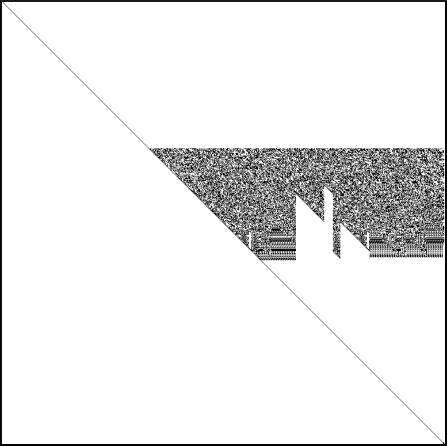
\includegraphics[width=0.24\linewidth]{Figures/UAR4JA.png}
    \caption{$L'$, $U'$ matrices of (2016,1008) example code in \cite{Mahdi2014} (left) and AR4JA $k$=1024 rate $1/2$ code (right).}
    \label{fig:Mahdi-LU}
\end{figure}    
In \cite{Cohen2009} the authors propose a hybrid approach, according to which the parity-check matrix is transformed in approximate lower-triangular form, as in R-U method. The parity bits are calculated using a mix of the direct and the R-U method: The first subvector $p_{1}$ of $g$ parity bits in R-U equation (\ref{eq:RU1}) is calculated from the the generator matrix $G$, according to the direct method. In this case, only the first $g$ columns of the submatrix $W_{n-k}$ in (\ref{eq:Wstructure}) need to be stored in encoder memory, avoiding thus the dense vector-matrix operations involving $\varphi^{-1}$. The paper focuses in IEEE 802.11an codes. For CCSDS AR4JA codes however, $g=4m$ and parameter $r$ is 8, 16, 32 for rates $1/2$, $2/3$, $3/4$ correspondingly, while $\varphi^{-1}$ is always $4m \times 4m$. No performance gain is therefore achievable from this method for CCSDS codes. On the contrary, memory requirements and critical path are adversely affected from the larger dense matrix involved. Also $T^{-1}$ is the identity matrix for AR4JA and the critical path is not affected.
                


\subsection{Packet level erasure codes}
Packet-level erasure coding has been proposed for many modern applications, such as edge computing \cite{Liang2020}, underwater acoustic sensor networks \cite{Geethu2015}, magnetic recording media \cite{Han2005}, hybrid broadcasting broadband television (HbbTV) \cite{Mattoussi2019} and delay tolerant networks (DTN) over deep space communication systems \cite{Alessi2020}. Joint use of erasure coding and bit-level FEC schemes in different scenarios has been studied in \cite{Courtade2011, Ostovari2015, Berger2008}.\par
The main focus of this thesis is on the implementation of encoders for the codes defined in \cite{CCSDS131.5}. The only implementation of the proposed codes is their integration into the the Interplanetary Overlay Network (ION) software suite \cite{ion}, which is a software implementation of the bundle protocol for Delay Tolerant Networks (DTN). In \cite{Alessi2020}, a multithreaded implementation of the ION libraries is proposed for better performance. However, the purely software approach proposed is expected to exert considerable strain on the on-board general purpose processor and mass memory subsystem of a space Software Defined Radio (SDR), which is typically responsible for these functions. Offloading these tasks to a small footprint hardware accelerator integrated into a FPGA is especially important in the case of microsats and cubesats and high data rate optical communications, to achieve reduced size, weight, power, and cost (SWaP-C). Typically, spacecraft subsystems already include FPGAs responsible for command and data handling (C\&DH) tasks and the recent trend is to fully utilize these devices for multiple combined functions \cite{Davarian2020}. Moreover, FPGA hardware acceleration of packet-level coding enables a very high speed data processing chain providing data rates in the scale of several Gbps.\par
